    \chapter{INTRODUCTION.}
    \lettrine[lines=2]{T}{HE arts and sciences have} become so extensive,
    that to facilitate their acquirement is of as much importance as to
    extend their boundaries. Illustration, if it does not shorten the time
    of study, will at least make it more agreeable. \textsc{This work} has
    a greater aim than mere illustration; we do not introduce colours for
    the purpose of entertainment, or to amuse \textit{by certain
    combinations of tint and form}, but to assist the mind in its
    researches after truth, to increase the facilities of instruction, and
    to diffuse permanent knowledge. If we wanted authorities to prove the
    importance and usefulness of geometry, we might quote every
    philosopher since the days of Plato. Among the Greeks, in ancient, as
    in the school of Pestalozzi and others in recent times, geometry was
    adopted as the best gymnastic of the mind. In fact, Euclid's Elements
    have become, by common consent, the basis of mathematical science all
    over the civilized globe. But this will not appear extraordinary, if
    we consider that this sublime science is not only better calculated
    than any other to call forth the spirit of inquity, to elevate the
    mind, and to strengthen the reasoning faculties, but also it forms the
    best introduction to most of the useful and important vocations of
    human life. Arithmetic, land-surveying, mensuration, engineering,
    navigation, mechanics, hydrostatics, pneumatics, optics, physical
    astronomy, \&c. are all dependent on the propositions ofgeometry. 

    Much however depends on the first communication of any science to a
    learner, though the best and most easy methods are seldom adopted.
    Propositions are placed before a student, who though having a
    sufficient understanding, is told just as much about them on entering
    at the very threshold of the science, as gives gives him a
    prepossession most unfavourable to his future study of this delightful
    subject; or the formalitites and paraphernalia of rigour are so
    ostentatiously put forward, as almost to hide the reality. Endless and
    perplexing repetitions, which do not confer greater exactitude on the
    reasoning, render the demonstrations involved and obscure, and conceal
    from the view of the student the consecution of evidence.'' Thus an
    aversion is created in the mind of the pupil, and a subject so
    calculated to improve the reasoning powers, and give the habit of
    close thinking, is degraded by a dry and rigid memory, To raise the
    curiosity, and to awaken the listless and dormant powers of younger
    minds should be the aim of every teacher; but where examples of
    excellence are wanting, the attempts to attain it are but few, while
    eminence excites attention and produces imitation. The object of this
    Work is to introduce a method of teaching geometry, which has been
    much approved of by many scientific men in this country, as well as
    in France and America. The plan here adopted forcibly appeals to the
    eye, the most sensitive and the most comprehensive of our external
    organs, and its pre-eminence to imprint it subject on the mind is
    supported by the incontrovertible maxim expressed in the well known
    words of Horace:- 
    \begin{quotation}
        \noindent\textit{Segnius irritant animos demissa per aurem \\
        Qu\`am qu\ae sunt oculis subjecta fidelibus} \\
        A feebler impress through the ear is made,\\
        Than what is by the faithful eye conveyed.
    \end{quotation}
    All language consists of representative signs, and those sins are the
    best which effect their purposes with the greatest precision and
    dispatch. Such for all common purposes are the audible signs called
    words, which are still considered as audible, whether addressed
    immediately to the ear, or through the medium of letteers to the ete.
    Geomerical science, the object of which is to show th erelative
    quantities of their parts by a process of reasoning called
    Demonstration. This reasoning has been generally carried on by words,
    letters, and black or uuncoloured diagrams; but as the use of coloured
    symbols, signs and diagrams in the linear arts and sciences, renders
    the process of reasoning more precise, and the attainment more
    expeditious, they have been in this instance accordingly adopted. 

    Such is the expedition of this enticing mode of communicating
    knowledge, that the Elements of Euclid can be acquired in less than
    one third the time usually emploted, and the retention by the memory
    is much more permanent; these facts have been ascertained by numerious
    experiments made by the invenror, and seveeral orhers who have adopted
    his plans. The particularsof which are few and obvious; the letters
    annexed to points, lines, or other parts of a diagram are in fact but
    arbitrary names, and represent them in the demonstration; instead of
    these, the parts being differently colouresd, are made to name
    themselves, for their forms in corresponding colours represent them in
    the demonstration. 

    In order to give a better idea of this system, and of the advantages
    gained by its adoption, let us take a right angled triangle, and
    express some of its properties both by colours and the method
    generally employed. 
    \newcommand{\cab}{
        
\begin{tikzpicture}[scale=2]
            \path[fill=red] (0,0) ++ (0.5,0) arc (0:36:0.5) -- (0,0);
        \end{tikzpicture}
    }
    \newcommand{\abc}{
        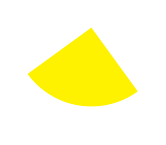
\begin{tikzpicture}[baseline=-6.0ex,rotate=216,scale=2]
            \path[fill=yellow] (0,0) ++ (0.5,0) arc (0:90:0.5) -- (0,0);
        \end{tikzpicture}
    }
    \newcommand{\bca}{
        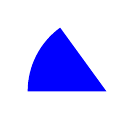
\begin{tikzpicture}[rotate=126,scale=2]
            \path[fill=blue] (0,0) ++ (0.5,0) arc (0:54:0.5) -- (0,0);
        \end{tikzpicture}
    }

    \begin{figure}
    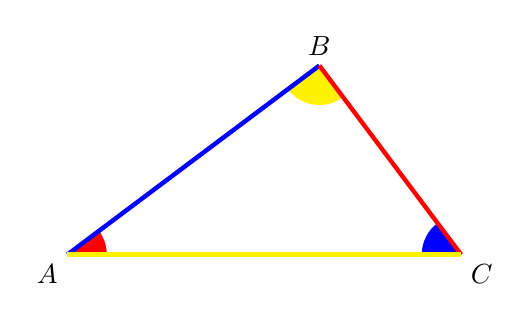
\begin{tikzpicture}
        \coordinate (A) at (0,0);
        \coordinate (B) at (3.2,2.4);
        \coordinate (C) at (5,0);
        \path[fill=red,ultra thick] (A) ++(0.5,0) arc (0:36:0.5) -- (A);
        \path[fill=yellow,ultra thick] (B) ++(-90+36:0.5) arc (-90+36:-180+36:0.5) -- (B);
        \path[fill=blue,ultra thick] (C) ++(-0.5,0) arc (180:90+36:0.5) -- (C);
        \node[below left ] at (A) {$A$};
        \node[above      ] at (B) {$B$};
        \node[below right] at (C) {$C$};
        \draw[blue,ultra thick]   (A) -- (B);
        \draw[red,ultra thick]    (B) -- (C);
        \draw[yellow,ultra thick] (C) -- (A);
    \end{tikzpicture}
    \end{figure}

    \begin{center}
        \textit{Some of the properties of the right angled triangle 
        \textrm{ABC}, expressed by the method generally employed.}
    \end{center}

    \begin{enumerate}
        \item The angle BAC, together with the angles BCA and ABC are 
            equal to two right angles, or twice the angle ABC. 
        \item The angle CAB added to the angle ACB will be equal to 
            the angle ABC. 
        \item The angle ABC is greater than either of the 
            angles BAC or BCA. 
        \item The angle BCA or the angle CAB is less than the 
            angle ABC. 
        \item If from the angle ABC, there be taken the angle BAC, 
            the remainder will be equal to the angle ACB. 
        \item The square of AC is equal to the sum of the squares 
            of AB and BC. 
    \end{enumerate}

    \begin{center}
        \textit{The same properties expressed by colouring 
        the different parts.}
    \end{center}

    \begin{enumerate}
        \item \[ \cab \plus \abc \plus \bca \equals 2\, \abc \equals \rightangles.\]
          That is, the red angle added to the yellow angle added to the blue angle, equal twice the yellow angle, equal two right angles. 
      \item \[\cab \plus \bca \equals \abc.\] 
          Or in words, the red angle added to the blue angle, equal the yellow angle. 
      \item \[\abc \greater \cab \text{ or } \greater \bca.\]
          The yellow angle is greater than either the red of blue angle. 
      \item \[\cab \text{ or } \bca \less\abc.\]
          Either the red or blue angle is less than the yellow angle.
      \item \[\abc \text{ minus } \bca \equals \cab.\]
          In other terms, the yellow angle made less by the blue angle equal the red angle. 
      \item \[\tikzhline[yellow]{1.2cm}^{2} \equals \tikzhline[blue]{1.2cm}^{2} \plus \tikzhline[red]{1.2cm}^{2}.\]
          That is, the square of the yellow line is equal to the sum of the squares of the blue and red lines. 
    \end{enumerate}

    In oral demonstrations we gain with colours this important advantage, the eye and the ear can be addressed at the same moment, so that for teavhing geometry, and other linear arts and sciences, in classes, the ststem is the best ever proposed, this is apparent from the examples just given. 

    Whence it is evident that a reference from the text to the diagram is more rapid and sure, by giving the forms and colours of the parts, or by naming the parts and their colours, than naming the parts and letters on the diagram. Besides the superior simplicity, this system is likewise conspicuous for concentration, and wholly excludes the injrious though prevalent practice of allowing the student to commit the demonstration to memory; until reason , and fact, and proof only make impressions on the understanding. 

    Again, when lecturing on the principles or properties of figures, if we mention the colour of the part or parts referred to, as in saying, the red angle, the blue line, or lines, \&c.~the part or parts thus names will be immediately seen by all in the class at the same instant; not so if we say the angle ABC, the triangle PFQ, the figure EGKt, and so on; for the letters must be traces one by one before the students arrange in their minds the particular magnitude reeferred to, which often occasions confusino and error, as well as lots of time. Also if the parts which are given as equal, have the same colours in any diagram, the mind will not wander from the object before it; that is, such an arrangement presents an ocular demonstration of the parts to be proved equal, and the learner retains the data throughout the whole of the reasoning. But whatever may be the advantages of the present plan, if it be not substituted for, it can always be made a powerful auxiliary to the other methods, for the purpose of introduction, or of a more speedt reminiscence, or of more permanent retention by the memory. 

    The experience of all who have formed systems to impress facts on the understanding, agree in proving that coloured representations, as pictures, cuts, diagrams, \&c.~are more easily fixed in the mind than mere sentences unmarked by any peculiarity. Curious as it may appear, poets seem to be aware of this fact more than mathematicians; many modern poets allude to this visible system of communicating knowledge, one of them has thus expressed himself: 
    \begin{quotation}
        Sounds which address the ear are lost and die\\
        In one short hour, but these which strike the eye,\\
        Live long upon the mind, the faithful sight\\
        Engraves the knowledge with a beam of light.
    \end{quotation}
    This perhaps may be reckoned the only improvement on which plain geometry has recerived since the dats of Euclid, and if there were any geometers of note before that time, Eclid's success has quite ecliped their memory, and even occasioned all good things of that kindto be assigned to him; like \AE sop among the writers of Fables. It may also be worthy of remark, as tangible diagrams afford only the medium through which geometry and other linear arts and scoences can be taught to the blind, this visible system is no less adapted to the exigencies of the deaf and dumb. 

